\documentclass[a4paper,11pt]{article}
\usepackage[spanish]{babel}
\usepackage[utf8]{inputenc}
\usepackage{hyperref}
\usepackage{graphicx}
\usepackage{siunitx}
\usepackage{cite}


\begin{document}
\title{Como la crisis del Covid-19 ha afectado a la calidad del aire}
\author{Yolanda Montilla Patón}
\maketitle


\begin{abstract}
 La pandemia de la COVID-19 se ha convertido en uno de los mayores retos que la humanidad se ha tenido que enfrentar en los últimos años. Se han realizado diversos estudios para determinar si la calidad del aire puede afectar a la propagación del virus y si las medidas tomadas por los gobiernos han sido determinante en un cambio en la calidad del aire. El siguiente artículo se encuentra localizado en mi plataforma Github:\href{https://github.com/yolandaMontilla/PROYECTO_FINAL.git}{URL}.

\ En dicho artículo se va intentar mostrar como esta crisis mundial ha sido un punto de inflexión de cómo un cambio radical de nuestra rutina diaria puede suponer grandes cambios en la calidad del aire y en la propagación de enfermedades.
\textbf{\\ Palabras clave:}
Calidad del aire, Corona virus, Gases de efecto hinvernadero.

\end{abstract}
\newpage

 \ INTRODUCCIÓN
\\ Los estudios científicos realizados en los primeros meses de 2020 sobre la realción entre aspectos atmosféricos y climáticos y propogación y contagio del corona virus no resultan concluyente y, en la mayoría de los casos, se trata de resultados preliminares.Wang et al.(2020b) han realizado un estudio donde analizan condiciones atmosféricas con la propagación del virus, tomando como referencia 429 ciudades de China dónde se observaron que el aumento de la humedad absoluta era una condicón desfavorable para la propagación.Wan, Tang, Feng y Lv(2020a) han elaborado un modelo de predicción de transmisión de la epidemia a partir de la temperatura y humedad relativa, según el cual aumento de 1ºC o 1\% de humedad, contribuyendo a reducir el número de reproducción efectiva de los casos. También se ha localiado una correlación con la calidad del aire , dónde ciudades con elebadores valores de partículas PM25 y dióxido de nitrógeno la pobleción es más propensa de contagiarse por el virus.
Diversos estudios todavía muy preliminares en China, Europa y Estados Unidos están relacionando la mortalidad ocasionada por la COVID-19 con la exposición a largo plazo a la contaminación atmosférica, tanto de partículas finas(PM25) como al dióxido de nitrogeno. Está relación deriva de la afección a los sistemas respiratorios e inmunitarios y eventualmente de la contribución a la transmisión del coronavirus, en la que las PM25 actuaran como vectores.
\\ Este artículo tiene como propósito, conocer la influencia que ha podido tener la climatología y la contaminación en la propagación del COVID-19 como referente el territorio Español y en busqueda de medidas de desescalamiento que no empeoren la calidad del aire.
\ \ \ \ \ \ \ \ \ \ \ \ \ \ \   \ \ \ \ \ \ \\ \ \ \ \ \ \ \ \ \ \ \ \ \ \   \ \ \ \ \ \ \\ \ \ \ \ \ \ \ \ \ \ \ \ \ \   \ \ \ \ \ \ \\ \ \ \ \ \ \ \ \ \ \ \ \ \ \   \ \ \ \ \ \ \\ \ \ \ \ \ \ \ \ \ \ \ \ \ \   \ \ \ \ \ \ \
 METODOLOGÍA
\\La recopilación de información a partir de los estudios, investigaciones y noticias publicadas, en la cual se han encontrado varios
inconvenientes. Por un lado, la afección de este nuevo virus a nivel planetario ha generado grandes volúmenes
de información, tanto a nivel académico/científico y de administraciones públicas, como a nivel
periodístico, en continua actualización, por lo que la validez de un estudio o una noticia puede que solo
sea de unas horas. Además, no siempre las conclusiones desarrolladas pasan por tener una fuente y una
metodología fiable, por lo que es necesario filtrar la información para evitar conclusiones erróneas. Es
necesario indicar que gran parte de los artículos científicos analizados en este trabajo, son “pre-prints”,
es decir, estudios que han sido publicados de manera temporal, y en su mayoría no revisados por pares,
que podrían ser modificados posteriormente. De ahí la necesidad de prudencia en la extracción de conclusiones
tras su lectura.
 \\ El análisis de los estudios analizados se han limitado en esta ocasión al NO2, por se la sustancia más directamente relacionada con el tráfico urbano. Se han recogido los datos oficiales de 129 de las 600 estaciones de medición de este contaminante existentes en España, correspondientes a las redes de las 26 principales ciudades, mayores de 150000 habitantes. la obtención de los datos se realizó a través de la página web diseñadas para publicar la información de las estaciones de control de la contaminación por las CCCAA.
\\El periodo de recopilación de la información ha comprendido entre el 1 de Marzo y el 30 de abril de 2020 y los mismos meses de los diez años anteriores(2010 a 2019), con el fin de reducir los sesgos meteorológicos y vacacinales debidos a las variaciones del teimpo y a la distribución enen cada año de los fines de semana y la Semana Santa.
\\Dentro de este periodo, que permite observar la variación a lo largo de marzo y abril de 2020 y
de ambos meses “tipo” (media de los años 2010 a 2019), se ha analizado separadamente el intervalo
entre los días 14 de marzo y 30 de abril, comparado con el correspondiente al promedio de la
década anterior, en el conjunto de las redes y en la estación orientada al tráfico más significativa
de cada ciudad, por su mayor concentración de NO2 y/o por su posición central.
\begin{figure}
\centering
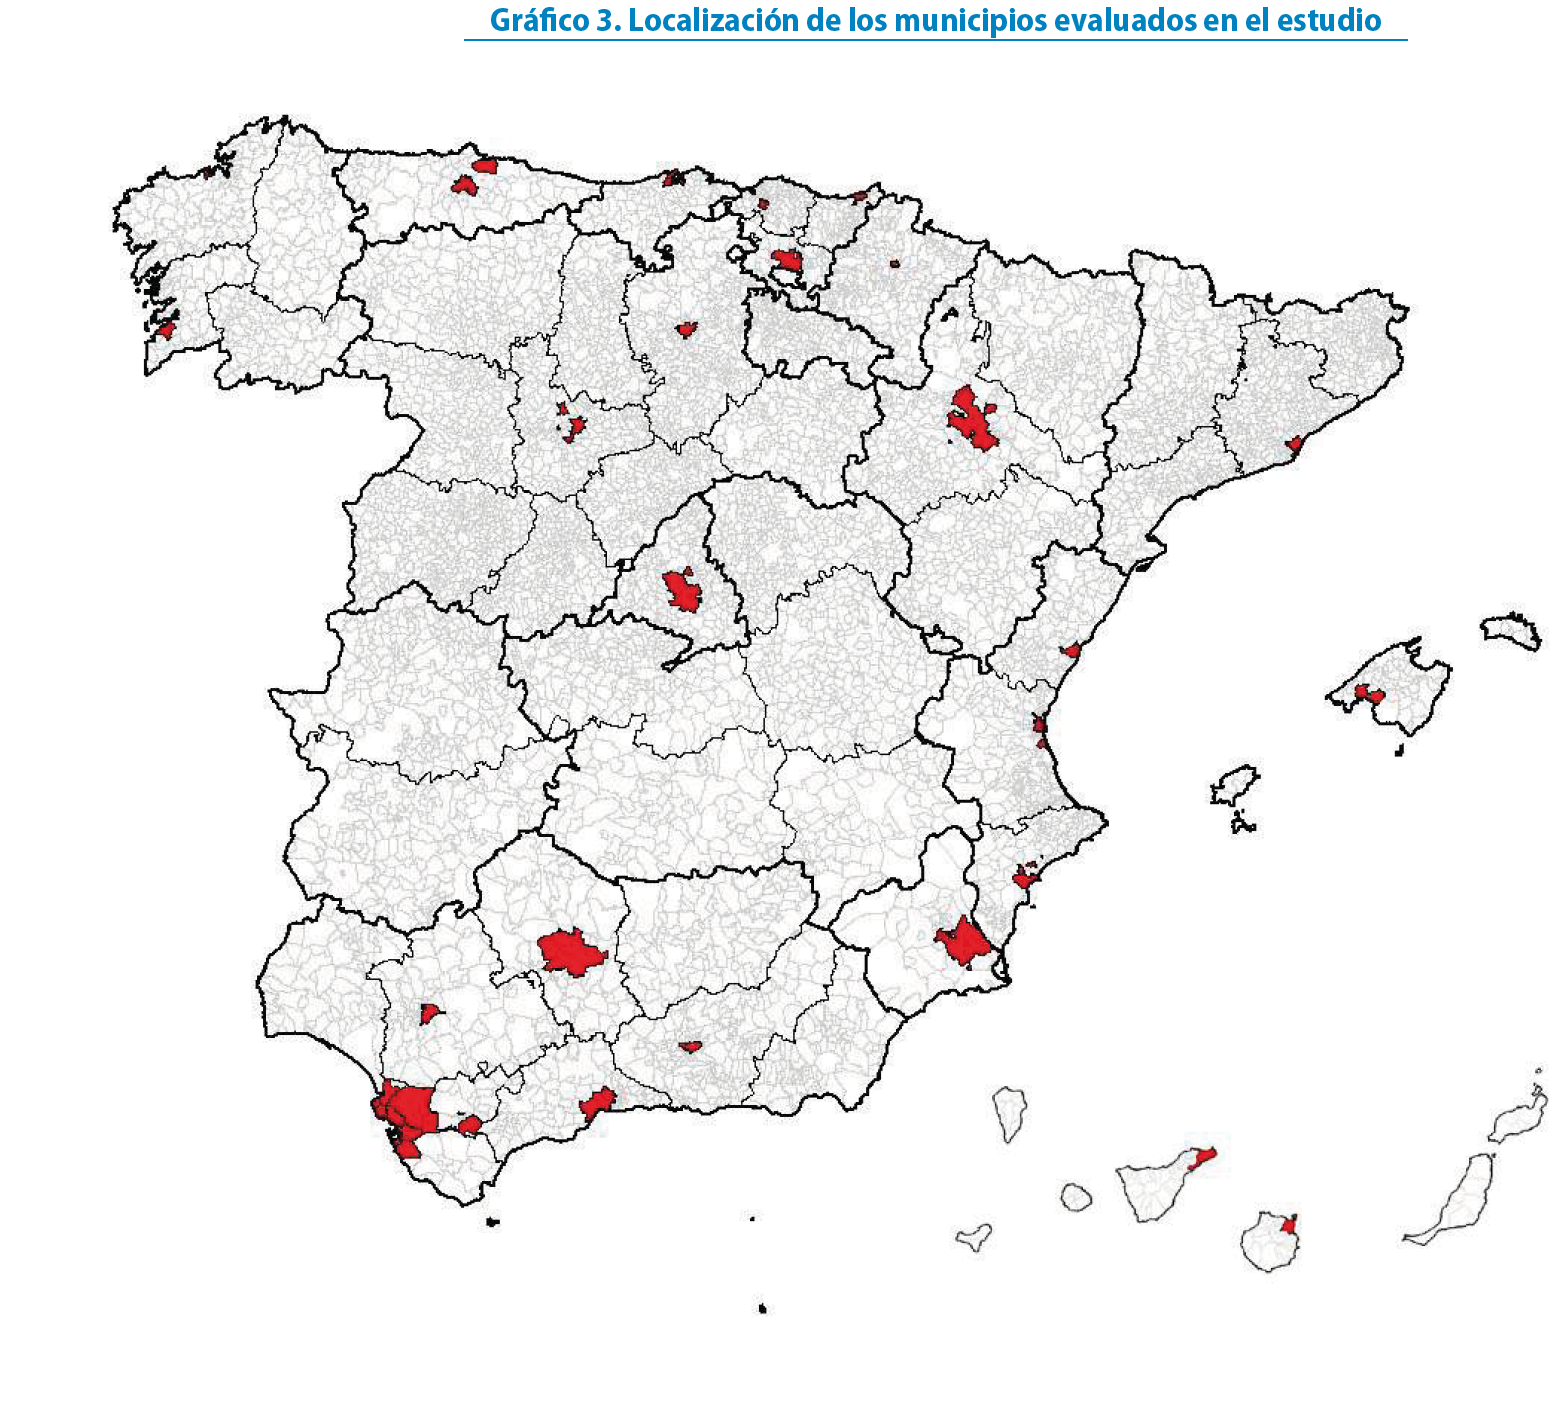
\includegraphics[width=6cm, height=6cm]{zonaestudio}
\caption{Zona de estudio}
\label{Figura1}
\end{figure}
\ \ \ \ \ \ \ \ \ \ \ \ \ \ \   \ \ \ \ \ \ \\ \ \ \ \ \ \ \ \ \ \ \ \ \ \   \ \ \ \ \ \ \\ \ \ \ \ \ \ \ \ \ \ \ \ \ \   \ \ \ \ \ \ \\ \ \ \ \ \ \ \ \ \ \ \ RESULTADOS
\\  Como resultado de las medidas de confinamiento social y limitación de la movilidad derivadas
del estado de alarma, en el periodo comprendido entre el 14 de marzo y el 30 de abril de 2020
se ha producido una reducción drástica de los niveles de NO2 en las redes de medición de las 26
ciudades consideradas, por comparación con el promedio del mismo periodo de los diez años
anteriores. En el conjunto de las 129 estaciones evaluadas, la reducción se cuantifica en un 58\%
de los niveles habituales.
\begin{figure}
\centering
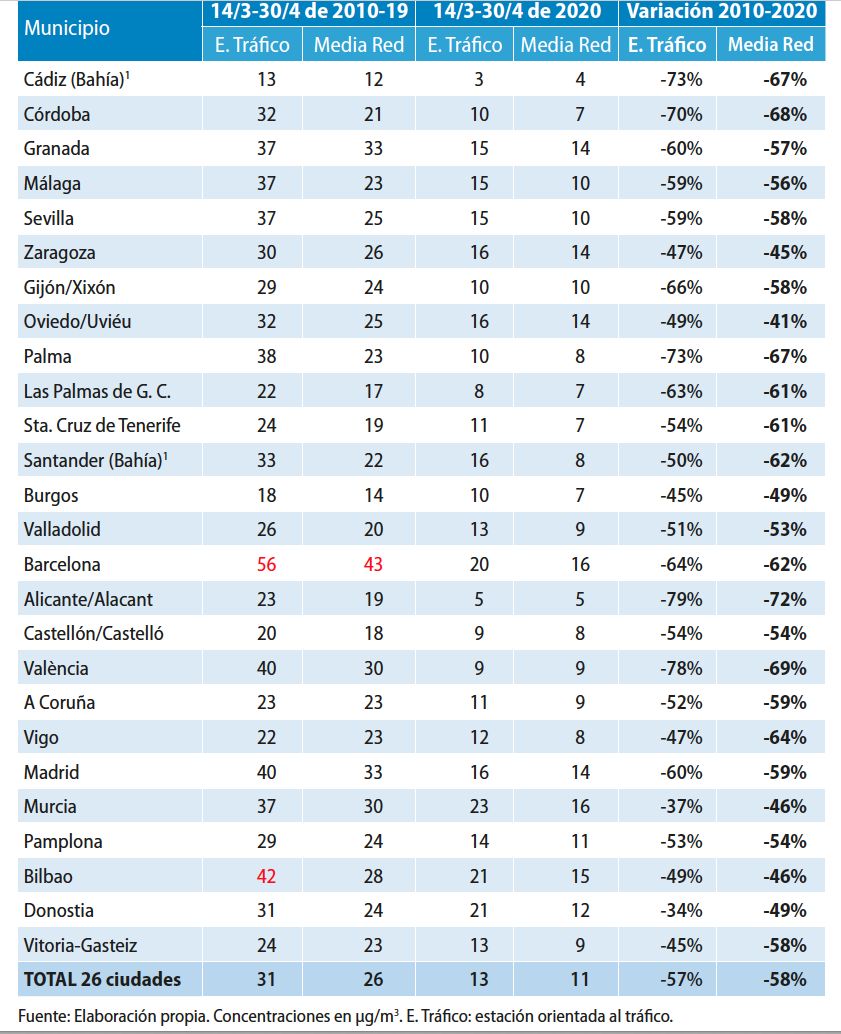
\includegraphics[width=15cm, height=15cm]{tabla}
\caption{Concentraciones NO2}
\label{Figura1}
\end{figure}
\\ El valor medio de NO2 de las redes urbanas entre el 14 de marzo y el 30 de abril de 2020 ha sido de 11 \si\micro\ g/m3 mientras el equivalente para el período 2010-2019 fue de 26 \si\micro\ g/m3. En el caso de las estaciones de tráfico más significativas de cada ciudad, la media de NO2 entre los pasados 14 de marzo y 30 de abril ha sido de 13 \si\micro\ g/m3, mientras en el período 2010-2019 fue de 31 \si\micro\ g/m3.
Los niveles de NO2 registrados durante el estado de alarma son los más bajos para la segunda
quincena de marzo y el mes de abril de la última década, en todas las ciudades analizadas.
Se mantienen además muy por debajo del valor límite anual y la guía a largo plazo de la OMS,
establecidos en 40 \si\micro\ g/m3, cuando en varias de las estaciones de tráfico de ciudades como
Barcelona, Bilbao, Granada, Madrid, Málaga, Murcia, Palma y València dicho umbral se supera
frecuentemente, especialmente durante marzo.
\\ Escasa contaminación atmosférica  en los meses de febrero y marzo es un dato a favor del posible menor efecto de la enfermedad.
Algunos estudios realizados en Europa, China y USA señalan que se ha detectado una tasa de mortalidad
mayor por la COVID-19 en aquellas regiones que presentan un mayor índice de contaminación del
aire. Zhu, Xie, Huang y Cao (2020) observan asociaciones significativamente positivas de PM 2,5, PM 10,
NO2 y O3 con casos confirmados por coronavirus. Wu, Nethery, Sabath, Braun y Dominici (2020) indican
que un aumento de solo 1 \si\micro\ g/m3 en PM 2,5 se asocia con un aumento del 8\% en la tasa de mortalidad de
COVID-19. Este hecho se ha observado también en Italia, donde la mayor parte de los fallecidos se han
registrado en la Lombardía, la región industrial por excelencia. Conticini, Fedriani y Caro (2020), en este
sentido concluye que los altos niveles de contaminación en el Norte de Italia deben considerarse como un
factor a tener en cuenta en la alta letalidad del coronavirus en esta región. En Francia las tasas han sido
mayores en Paris y en los departamentos de la mitad septentrional o cercanos a la frontera con Alemania.
\ \ \ \ \ \ \ \ \ \ \ \ \ \ \   \ \ \ \ \ \ \\ \ \ \ \ \ \ \ \ \ \ \ \ \ \   \ \ \ \ \ \ \\ \ \ \ \ \ \ \ \ \ \ \ \ \ \   \ \ \ \ \ \ \\ \ \ \ \ \ \ \ \ \ \ \ CONCLUSIONES Y RECOMENDACIONES
\\ El NO2 provoca cada año en España alrededor de 7.000 muertes prematuras, según el Instituto
de Salud Carlos III y la Agencia Europea de Medio Ambiente. Es un gas irritante que agrava
las enfermedades respiratorias y merma la resistencia a las infecciones, al inhibir la respuesta
inmunológica de los pulmones, por lo que su drástica reducción es una buena noticia, en el
contexto de emergencia sanitaria actual. Diversos estudios ya han apuntado a la influencia de
la contaminación atmosférica crónica en la gravedad de las patologías respiratorias asociadas
a la COVID-19.
\\ La crisis de la COVID-19 demuestra que la reducción estructural del tráfico motorizado y los
cambios en las pautas de movilidad son las mejores herramientas para mejorar la calidad del
aire en las ciudades. La dramática situación creada por la pandemia viene a corroborar algo en
lo que viene insistiendo desde hace años la comunidad científica: que la reducción del tráfico
en las ciudades tiene claros efectos en la disminución de la contaminación, algo que a su vez
supone una importante mejora de la salud pública.
Paradójicamente, la salida de la crisis podría conllevar el aumento de la contaminación atmosférica,
incluso por encima de los niveles precedentes. Las obligadas medidas de seguridad
y distanciamiento físico que nos acompañarán durante meses tras el confinamiento, van a hacer
complicado el funcionamiento del transporte público en la forma habitual.
\\ Ante todo, es necesario mantener algunas “buenas prácticas” de la crisis que limitan la necesidad
de desplazamientos, adaptadas a un escenario de paulatina normalización, como son
la compra de proximidad, el teletrabajo como opción laboral voluntaria, una administración
electrónica más eficiente o el escalonamiento de los horarios laborales. Se trata de opciones
compatibles con el distanciamiento social que permitirían manejar de forma más racional el
acceso de la ciudadanía a los servicios y ciertos trabajos.
\textbf{\\ Gestión de la demanda de movilidad:}
\begin{itemize}
\item Reducir las necesidades de transporte, fomentando el teletrabajo, la compra de proximidad
y la administración electrónica.
\item Reducir al máximo la aparición de horas punta, flexibilizando los horarios y escalonando
la entrada y salida a los puestos de trabajo y servicios.
\item Campañas a favor de los desplazamientos caminando y en bicicleta en trayectos de
menos de 6 kilómetros.
\item Crear zonas verdes temporales para evitar aglomeraciones en parques y jardines y reducir
desplazamientos a lugares de recreo.
\end{itemize}
\textbf{\\ Fomento de los desplazamientos a pie:}
\begin{itemize}
\item Ampliación de aceras para facilitar el distanciamiento físico. Se puede realizar a costa del
espacio de la calzada o de las bandas de aparcamiento.
\item Establecimiento de calles compartidas (sin separación calzada-acera) y zonas con prioridad
peatonal, en las calles en las que no se puedan ampliar las aceras, donde las personas
tendrán prioridad para caminar por la calzada.
\item Ubicación de terrazas, contenedores y aparcamiento de motos preferentemente en la
calzada y no en la acera.
\item Restricción de la circulación de vehículos a motor en torno a los centros docentes, en las
horas de entrada y salida del alumnado.
\item Programación semafórica para reducir los tiempos de espera en los pasos de peatones,
evitando las aglomeraciones de personas.
\end{itemize}
\textbf{\\ Fomento de los desplazamientos a pie:}
\begin{itemize}
\item Implantar redes y corredores ciclistas de emergencia.
\item Promover aparcamientos seguros en puntos estratégicos (intercambiadores de transporte
público, edificios administrativos, estaciones de tren).
\item Implantar estacionamientos de bicicletas en los centros de trabajo.
\item Plan de ayudas para la adquisición y reparación de bicicletas por particulares.
\end{itemize}
\textbf{\\ Potenciar el transporte público:}
\begin{itemize}
\item Ampliar el número y dimensión de los carriles bus en las zonas urbanas y priorizarlos
semafóricamente.
\item Habilitar carriles bus en todas las autovías y autopistas de acceso a las grandes ciudades.
\item Ley de financiación del transporte público que garantice su viabilidad, con medidas de
financiación de urgencia.
\item Moratoria en la ampliación de autopistas y autovías, destinando su presupuesto para
implementar medidas que favorezcan el transporte público.
\item Moratoria en la ampliación de autopistas y autovías, destinando su presupuesto para
implementar medidas que favorezcan el transporte público.
\end{itemize}
\newpage
BIBLIOGRAFÍA
\bibliography{bibliografia}
\bibliographystyle{plain}
\cite[en2020efectos]
\cite[cantos2020aspectos]
 \\ RECURSOS
\begin{itemize}
\item https://www.easp.es/web/coronavirusysaludpublica/efecto-de-la-pandemia-de-covid-19-en-la-calidad-del-aire-impacto-en-la-salud-respiratoria/
\item https://www.easp.es/web/coronavirusysaludpublica/el-clima-y-la-contaminacion-modifican-la-transmision-del-sars-cov-2/
\end{itemize}
\end{document}